
%% Support sites:
%% http://www.michaelshell.org/tex/ieeetran/
%% http://www.ctan.org/pkg/ieeetran
%% and
%% http://www.ieee.org/


% *** Authors should verify (and, if needed, correct) their LaTeX system  ***
% *** with the testflow diagnostic prior to trusting their LaTeX platform ***
% *** with production work. The IEEE's font choices and paper sizes can   ***
% *** trigger bugs that do not appear when using other class files.       ***                          ***
% The testflow support page is at:
% http://www.michaelshell.org/tex/testflow/



\documentclass[conference,compsoc]{IEEEtran}
% Some/most Computer Society conferences require the compsoc mode option,
% but others may want the standard conference format.
%
% If IEEEtran.cls has not been installed into the LaTeX system files,
% manually specify the path to it like:
% \documentclass[conference,compsoc]{../sty/IEEEtran}





% Some very useful LaTeX packages include:
% (uncomment the ones you want to load)

% *** CITATION PACKAGES ***
%
\ifCLASSOPTIONcompsoc
  % IEEE Computer Society needs nocompress option
  % requires cite.sty v4.0 or later (November 2003)
  \usepackage[nocompress]{cite}
\else
  % normal IEEE
  \usepackage{cite}
\fi
% cite.sty was written by Donald Arseneau
% V1.6 and later of IEEEtran pre-defines the format of the cite.sty package
% \cite{} output to follow that of the IEEE. Loading the cite package will
% result in citation numbers being automatically sorted and properly
% "compressed/ranged". e.g., [1], [9], [2], [7], [5], [6] without using
% cite.sty will become [1], [2], [5]--[7], [9] using cite.sty. cite.sty's
% \cite will automatically add leading space, if needed. Use cite.sty's
% noadjust option (cite.sty V3.8 and later) if you want to turn this off
% such as if a citation ever needs to be enclosed in parenthesis.
% cite.sty is already installed on most LaTeX systems. Be sure and use
% version 5.0 (2009-03-20) and later if using hyperref.sty.
% The latest version can be obtained at:
% http://www.ctan.org/pkg/cite
% The documentation is contained in the cite.sty file itself.
%
% Note that some packages require special options to format as the Computer
% Society requires. In particular, Computer Society  papers do not use
% compressed citation ranges as is done in typical IEEE papers
% (e.g., [1]-[4]). Instead, they list every citation separately in order
% (e.g., [1], [2], [3], [4]). To get the latter we need to load the cite
% package with the nocompress option which is supported by cite.sty v4.0
% and later.





% *** GRAPHICS RELATED PACKAGES ***
\usepackage{color}
%
\ifCLASSINFOpdf
\usepackage[pdftex]{graphicx}
  % declare the path(s) where your graphic files are
  % \graphicspath{{../pdf/}{../jpeg/}}
  % and their extensions so you won't have to specify these with
  % every instance of \includegraphics
  % \DeclareGraphicsExtensions{.pdf,.jpeg,.png}
\else
  % or other class option (dvipsone, dvipdf, if not using dvips). graphicx
  % will default to the driver specified in the system graphics.cfg if no
  % driver is specified.
  % \usepackage[dvips]{graphicx}
  % declare the path(s) where your graphic files are
  % \graphicspath{{../eps/}}
  % and their extensions so you won't have to specify these with
  % every instance of \includegraphics
  % \DeclareGraphicsExtensions{.eps}
\fi
% graphicx was written by David Carlisle and Sebastian Rahtz. It is
% required if you want graphics, photos, etc. graphicx.sty is already
% installed on most LaTeX systems. The latest version and documentation
% can be obtained at:
% http://www.ctan.org/pkg/graphicx
% Another good source of documentation is "Using Imported Graphics in
% LaTeX2e" by Keith Reckdahl which can be found at:
% http://www.ctan.org/pkg/epslatex
%
% latex, and pdflatex in dvi mode, support graphics in encapsulated
% postscript (.eps) format. pdflatex in pdf mode supports graphics
% in .pdf, .jpeg, .png and .mps (metapost) formats. Users should ensure
% that all non-photo figures use a vector format (.eps, .pdf, .mps) and
% not a bitmapped formats (.jpeg, .png). The IEEE frowns on bitmapped formats
% which can result in "jaggedy"/blurry rendering of lines and letters as
% well as large increases in file sizes.
%
% You can find documentation about the pdfTeX application at:
% http://www.tug.org/applications/pdftex





% *** MATH PACKAGES ***
%
%\usepackage{amsmath}
% A popular package from the American Mathematical Society that provides
% many useful and powerful commands for dealing with mathematics.
%
% Note that the amsmath package sets \interdisplaylinepenalty to 10000
% thus preventing page breaks from occurring within multiline equations. Use:
%\interdisplaylinepenalty=2500
% after loading amsmath to restore such page breaks as IEEEtran.cls normally
% does. amsmath.sty is already installed on most LaTeX systems. The latest
% version and documentation can be obtained at:
% http://www.ctan.org/pkg/amsmath





% *** SPECIALIZED LIST PACKAGES ***
%
%\usepackage{algorithmic}
% algorithmic.sty was written by Peter Williams and Rogerio Brito.
% This package provides an algorithmic environment fo describing algorithms.
% You can use the algorithmic environment in-text or within a figure
% environment to provide for a floating algorithm. Do NOT use the algorithm
% floating environment provided by algorithm.sty (by the same authors) or
% algorithm2e.sty (by Christophe Fiorio) as the IEEE does not use dedicated
% algorithm float types and packages that provide these will not provide
% correct IEEE style captions. The latest version and documentation of
% algorithmic.sty can be obtained at:
% http://www.ctan.org/pkg/algorithms
% Also of interest may be the (relatively newer and more customizable)
% algorithmicx.sty package by Szasz Janos:
% http://www.ctan.org/pkg/algorithmicx




% *** ALIGNMENT PACKAGES ***
%
%\usepackage{array}
% Frank Mittelbach's and David Carlisle's array.sty patches and improves
% the standard LaTeX2e array and tabular environments to provide better
% appearance and additional user controls. As the default LaTeX2e table
% generation code is lacking to the point of almost being broken with
% respect to the quality of the end results, all users are strongly
% advised to use an enhanced (at the very least that provided by array.sty)
% set of table tools. array.sty is already installed on most systems. The
% latest version and documentation can be obtained at:
% http://www.ctan.org/pkg/array


% IEEEtran contains the IEEEeqnarray family of commands that can be used to
% generate multiline equations as well as matrices, tables, etc., of high
% quality.




% *** SUBFIGURE PACKAGES ***
%\ifCLASSOPTIONcompsoc
%  \usepackage[caption=false,font=footnotesize,labelfont=sf,textfont=sf]{subfig}
%\else
%  \usepackage[caption=false,font=footnotesize]{subfig}
%\fi
% subfig.sty, written by Steven Douglas Cochran, is the modern replacement
% for subfigure.sty, the latter of which is no longer maintained and is
% incompatible with some LaTeX packages including fixltx2e. However,
% subfig.sty requires and automatically loads Axel Sommerfeldt's caption.sty
% which will override IEEEtran.cls' handling of captions and this will result
% in non-IEEE style figure/table captions. To prevent this problem, be sure
% and invoke subfig.sty's "caption=false" package option (available since
% subfig.sty version 1.3, 2005/06/28) as this is will preserve IEEEtran.cls
% handling of captions.
% Note that the Computer Society format requires a sans serif font rather
% than the serif font used in traditional IEEE formatting and thus the need
% to invoke different subfig.sty package options depending on whether
% compsoc mode has been enabled.
%
% The latest version and documentation of subfig.sty can be obtained at:
% http://www.ctan.org/pkg/subfig




% *** FLOAT PACKAGES ***
%
%\usepackage{fixltx2e}
% fixltx2e, the successor to the earlier fix2col.sty, was written by
% Frank Mittelbach and David Carlisle. This package corrects a few problems
% in the LaTeX2e kernel, the most notable of which is that in current
% LaTeX2e releases, the ordering of single and double column floats is not
% guaranteed to be preserved. Thus, an unpatched LaTeX2e can allow a
% single column figure to be placed prior to an earlier double column
% figure.
% Be aware that LaTeX2e kernels dated 2015 and later have fixltx2e.sty's
% corrections already built into the system in which case a warning will
% be issued if an attempt is made to load fixltx2e.sty as it is no longer
% needed.
% The latest version and documentation can be found at:
% http://www.ctan.org/pkg/fixltx2e


%\usepackage{stfloats}
% stfloats.sty was written by Sigitas Tolusis. This package gives LaTeX2e
% the ability to do double column floats at the bottom of the page as well
% as the top. (e.g., "\begin{figure*}[!b]" is not normally possible in
% LaTeX2e). It also provides a command:
%\fnbelowfloat
% to enable the placement of footnotes below bottom floats (the standard
% LaTeX2e kernel puts them above bottom floats). This is an invasive package
% which rewrites many portions of the LaTeX2e float routines. It may not work
% with other packages that modify the LaTeX2e float routines. The latest
% version and documentation can be obtained at:
% http://www.ctan.org/pkg/stfloats
% Do not use the stfloats baselinefloat ability as the IEEE does not allow
% \baselineskip to stretch. Authors submitting work to the IEEE should note
% that the IEEE rarely uses double column equations and that authors should try
% to avoid such use. Do not be tempted to use the cuted.sty or midfloat.sty
% packages (also by Sigitas Tolusis) as the IEEE does not format its papers in
% such ways.
% Do not attempt to use stfloats with fixltx2e as they are incompatible.
% Instead, use Morten Hogholm'a dblfloatfix which combines the features
% of both fixltx2e and stfloats:
%
% \usepackage{dblfloatfix}
% The latest version can be found at:
% http://www.ctan.org/pkg/dblfloatfix




% *** PDF, URL AND HYPERLINK PACKAGES ***
%
%\usepackage{url}
% url.sty was written by Donald Arseneau. It provides better support for
% handling and breaking URLs. url.sty is already installed on most LaTeX
% systems. The latest version and documentation can be obtained at:
% http://www.ctan.org/pkg/url
% Basically, \url{my_url_here}.




% *** Do not adjust lengths that control margins, column widths, etc. ***
% *** Do not use packages that alter fonts (such as pslatex).         ***
% There should be no need to do such things with IEEEtran.cls V1.6 and later.
% (Unless specifically asked to do so by the journal or conference you plan
% to submit to, of course. )


% correct bad hyphenation here
\hyphenation{op-tical net-works semi-conduc-tor}


\usepackage[utf8]{inputenc}
\usepackage[T1]{fontenc}
\usepackage{lmodern}


% An example of a floating figure using the graphicx package.
% Note that \label must occur AFTER (or within) \caption.
% For figures, \caption should occur after the \includegraphics.
% Note that IEEEtran v1.7 and later has special internal code that
% is designed to preserve the operation of \label within \caption
% even when the captionsoff option is in effect. However, because
% of issues like this, it may be the safest practice to put all your
% \label just after \caption rather than within \caption{}.
%
% Reminder: the "draftcls" or "draftclsnofoot", not "draft", class
% option should be used if it is desired that the figures are to be
% displayed while in draft mode.
%
%\begin{figure}[!t]
%\centering
%\includegraphics[width=2.5in]{myfigure}
% where an .eps filename suffix will be assumed under latex,
% and a .pdf suffix will be assumed for pdflatex; or what has been declared
% via \DeclareGraphicsExtensions.
%\caption{Simulation results for the network.}
%\label{fig_sim}
%\end{figure}

% Note that the IEEE typically puts floats only at the top, even when this
% results in a large percentage of a column being occupied by floats.


% An example of a double column floating figure using two subfigures.
% (The subfig.sty package must be loaded for this to work.)
% The subfigure \label commands are set within each subfloat command,
% and the \label for the overall figure must come after \caption.
% \hfil is used as a separator to get equal spacing.
% Watch out that the combined width of all the subfigures on a
% line do not exceed the text width or a line break will occur.
%
%\begin{figure*}[!t]
%\centering
%\subfloat[Case I]{\includegraphics[width=2.5in]{box}%
%\label{fig_first_case}}
%\hfil
%\subfloat[Case II]{\includegraphics[width=2.5in]{box}%
%\label{fig_second_case}}
%\caption{Simulation results for the network.}
%\label{fig_sim}
%\end{figure*}
%
% Note that often IEEE papers with subfigures do not employ subfigure
% captions (using the optional argument to \subfloat[]), but instead will
% reference/describe all of them (a), (b), etc., within the main caption.
% Be aware that for subfig.sty to generate the (a), (b), etc., subfigure
% labels, the optional argument to \subfloat must be present. If a
% subcaption is not desired, just leave its contents blank,
% e.g., \subfloat[].


% An example of a floating table. Note that, for IEEE style tables, the
% \caption command should come BEFORE the table and, given that table
% captions serve much like titles, are usually capitalized except for words
% such as a, an, and, as, at, but, by, for, in, nor, of, on, or, the, to
% and up, which are usually not capitalized unless they are the first or
% last word of the caption. Table text will default to \footnotesize as
% the IEEE normally uses this smaller font for tables.
% The \label must come after \caption as always.
%
%\begin{table}[!t]
%% increase table row spacing, adjust to taste
%\renewcommand{\arraystretch}{1.3}
% if using array.sty, it might be a good idea to tweak the value of
% \extrarowheight as needed to properly center the text within the cells
%\caption{An Example of a Table}
%\label{table_example}
%\centering
%% Some packages, such as MDW tools, offer better commands for making tables
%% than the plain LaTeX2e tabular which is used here.
%\begin{tabular}{|c||c|}
%\hline
%One & Two\\
%\hline
%Three & Four\\
%\hline
%\end{tabular}
%\end{table}


% Note that the IEEE does not put floats in the very first column
% - or typically anywhere on the first page for that matter. Also,
% in-text middle ("here") positioning is typically not used, but it
% is allowed and encouraged for Computer Society conferences (but
% not Computer Society journals). Most IEEE journals/conferences use
% top floats exclusively.
% Note that, LaTeX2e, unlike IEEE journals/conferences, places
% footnotes above bottom floats. This can be corrected via the
% \fnbelowfloat command of the stfloats package.

\begin{document}
%
% paper title
% Titles are generally capitalized except for words such as a, an, and, as,
% at, but, by, for, in, nor, of, on, or, the, to and up, which are usually
% not capitalized unless they are the first or last word of the title.
% Linebreaks \\ can be used within to get better formatting as desired.
% Do not put math or special symbols in the title.
\title{Human-Robot Interaction by Prediction of Human Actions\\ Autonomous Systems - Instituto Superior T\'{e}cnico}


% author names and affiliations
% use a multiple column layout for up to three different
% affiliations
\author{\IEEEauthorblockN{João Rocha e Melo}
\IEEEauthorblockA{70831}
\and
\IEEEauthorblockN{Filipe Costa}
\IEEEauthorblockA{73055}
\and
\IEEEauthorblockN{Diogo Maximino}
\IEEEauthorblockA{73110}
\and
\IEEEauthorblockN{João Almeida}
\IEEEauthorblockA{73198}
\and
\IEEEauthorblockN{João Severino}
\IEEEauthorblockA{73608}}

\maketitle

% As a general rule, do not put math, special symbols or citations
% in the abstract
\begin{abstract}
Within the framework of this project, in order to be able to have an interaction between the human user and the robot it was used a Kinect camera, the Scout base robot and the Katana arm.\\
The Kinect was used for the system to learn informations about the outer world, in this case to learn about positions and movements of the user, with help of a skeleton-tracker software.\\
For controlling the Scout a simple controller was created that allows the robot to move forward and backwards.\\
The Katana represents one big part of the robot interaction, given that the robotic arm has a lot of movement possibilities being therefore possible to replicate human-like movements/behaviours.\\
Between the input information coming from the Kinect and the output provided by the Scout and Katana a machine learning algorithm was developed to introduce the prevision part of the project to the whole system.
\end{abstract}

% no keywords


% For peer review papers, you can put extra information on the cover
% page as needed:
% \ifCLASSOPTIONpeerreview
% \begin{center} \bfseries EDICS Category: 3-BBND \end{center}
% \fi
%
% For peerreview papers, this IEEEtran command inserts a page break and
% creates the second title. It will be ignored for other modes.
\IEEEpeerreviewmaketitle

\section{Introduction}
The main goal of this project is to make a mobile robot display human-aware behaviours, based on the predicted behaviours of the human the robot is interacting with. 

% Here insert Theorectical Introduction


The Human Robot Interaction problem was approached with certain assumptions/approximations as a basis for our work. These are the assumptions that our project tries to prove: 

\begin{itemize}
\item People tend to interact with other people with well defined and clear sequences of movements and gestures;
\item The sequences of gestures tend to be similar for a given situation even across different people;
\item A Machine Learning Classifier will be able to capture information that would be too hard to explicitly program. $\rightarrow$ This system should have improved results over explicitly programmed solutions;
\end{itemize}

With these items in mind we developed a setup to test our approach. The robot detected gestures and movements of the user and based on the sequence tried to predict what next action should take.





\section{Material and Software Used}
For this project it was allowed to use a RGB-D camera and a mobile robot. The camera used was the Kinect and the mobile robot consists of a robotic base, Scout, and a robotic arm, Katana.\\

\subsection{Kinect}
Along with the Kinect camera, a ROS package called \textit{openni-tracker} was used to detect the human body. This package gives as output the position of several points of the user's body, such as: head, neck, shoulders, elbows, hands, torso, hips, knees and feet.
\begin{figure}[!h]
	\centering
		\includegraphics[scale=0.5]{./Skeleton_tracker}
	\caption{Points given by the \textit{openni-tracker}}
\end{figure}\\

\subsection{Katana}
\label{Material: Katana}
To operate the Katana we used the already existent ROS package, \textit{Katana Native Interface}. Using this driver it is possible to power off the motors, allowing manual set of the robot positions and a reading of the maximum and minimum values for the different joints. After concluding this step it is possible to send commands to the Katana with the value for each joint position as well as the time to execute the movement. Sending a combination of these commands, it is possible for the Katana to reproduce simple human-like gestures.\\

\subsection{Scout}
Having in mind that the Scout is already an older robot it is difficult to find a ROS package which allows the inclusion of Scout in it, therefore we chose to program our own controller using the Scout driver. The driver allows us to read the odometry of the robot. In addition to the odometry, knowing that Scout receives as a command a distance to a certain place, the programmed controller is based on the comparison of the odometry with the distance that the robot was told to move. Although we only implemented this controller for one dimension movements, because there were some troubles with the odometry measurements associated with the needed rotation for the two dimensional movement. Considering that the main goal of the project is not to have a perfectly mobile robot, we decided to leave this point for future refinement of the system.\\

\section{Our Structure}
\begin{figure}[!h]
    \centering
    \includegraphics[width=0.5\columnwidth]{./OurStructure.png}
    \caption{Adele's Structure}
    \label{fig:adele_structure}
\end{figure}

\subsection{Kinect Node: Gestures}
Gesture recognition can be performed by tracking the movements of the different parts of the body. Once a stable detection of the joints is made, following them is the starting point towards the gesture recognition. 

Using a tracking software, the stable detection was achieved using a median filter of 5 samples.  Extracting these features from the image allow the construction of small movements and/or complete gestures. From points representing joints it's straightforward to use vectors to represent parts of the body like arm and forearm. Relations between them, such as angles or distances perform a good way to detect movements independent from the camera's referential.  

Not only the dislocation of the joints positions but also features as velocities and accelerations are detected. This way small movements are recognize as opening and closing the forearm or the arm moving up as well as moving down. In this work the goal is the prevision of gestures, therefore it is fundamental to detect small movements from which the gesture is built. The small movements include the variation position of the hand regarding the elbow, the position of the elbow regarding the torso, the amplitude between forearm and arm and the amplitude of the arm regarding the torso. More than one gesture can be built using the same small movements.

In order to help the system recognizing more accurately the gestures we included in this work the detection of waving, calling and handing gestures using the movements previously described.

Furthermore, it is also included detection of the position of the person in the world frame and the person's velocity. As for simplifying purposes it was decided to only work in one spatial dimension, the position is detected by computing the distance between the person and the kinect camera based on the mean of the points given by the hips, neck and torso. 

\subsection{Action Node: Katana \& Scout Movement}
\subsubsection{Katana}
As mentioned in section \ref{Material: Katana} with help of the \textit{ROS} package \textit{Katana Native Interface} it is possible to power-off the motors of the robotic arm while keeping the robot communicating with the computer.

While the motors are off, one can move the arm to the desired positions and afterwards read the values of the joint positions. Doing this repeatedly using all the desired positions, it is possible to program movement sequences, creating a gesture. After having each step of the movement, we programmed the maximum time for executing each step of the gesture. As well as for the positions, these maximum times were empirically determined. In the end of each movement, Katana goes to a defined default position.

Using this line of thought we created the following gestures: high-five, low-five, clap, wave, pass the slide and grab.

Since Katana as 7 degrees of freedom (6 joints and the gripper), the structures sent to Katana are a vector with 7 entries.
\begin{center}
General structure:
$\left[ Joint1, Joint2, Joint3, Joint4, Joint5, Joint6, Gripper\right]$\\
\end{center}
Using as an example the gesture "wave", the maximum time for reaching each position and the position goal sequence are given by:
\begin{center}
Maximum time:
$\left[5, 1.3, 1.3, 1.3, 5\right]$\\
\end{center}
\begin{table}[!h]
\centering
\begin{tabular}{lc}
Position 1: & {[}-1.85, 1.57, 0.175, -0.35, -1.57, 0.175, 0.175{]} \\
Position 2: & {[}-1.85, 1.57, 0.175, 0.35, -1.57, 0.175, 0.175{]}  \\
Position 3: & {[}-1.85, 1.57, 0.175, -0.35, -1.57, 0.175, 0.175{]} \\
Position 4: & {[}-1.85, 1.57, 0.175, 0.35, -1.57, 0.175, 0.175{]}  \\
Position 5: & Default Position                                    
\end{tabular}
\caption{Wave Sequence}
\label{wave}
\end{table}

Looking at the table~\ref{wave} we can observe that in this movement the only joint that changes its position is Joint 4, similar to the human gesture where the only joint that moves while waving is the elbow joint.

\subsubsection{Scout}
The Scout robot is a two wheel, two motor differential drive robot, that means that for controlling the robot, one needs a linear and an angular velocity. One can translate these two velocities to the velocities of each wheel, by using following equations:
\begin{equation}
v_{lin} = \frac{(\omega_{right}+\omega_{left})r}{2} \\
\end{equation}
\begin{equation}
v_{ang} = \omega = \frac{(\omega_{right}-\omega_{left})r}{2d}
\end{equation}
Where $r$ represents the radius of the wheel, and $d$ the distance between wheels.
As it can be seen in figure \ref{fig:scout_axis} our robot has two degrees of freedom, but since the movement of the robot isn't the main point of this project, we assume, as a proof of concept, to only move in the \textit{x}-axis (forwards and backwards).

The implemented controller receives as an input a dislocation. The idea of having as input a final position in the world map, is a possible improvement for future work, but requires the robot tracking by the Kinect Node.

\begin{figure}[!h]
    \centering
    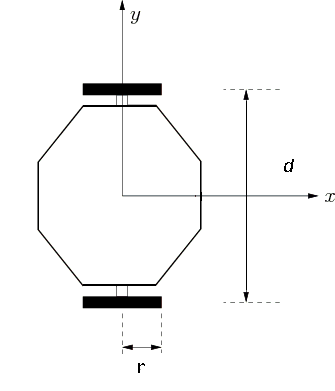
\includegraphics[width=0.5\columnwidth]{./ScoutAxis.png}
    \caption{Scout Axis}
    \label{fig:scout_axis}
\end{figure}
The control loop that we implemented looks as shown in figure \ref{fig:scout_loop}.
\begin{figure}[!h]
    \centering
    \includegraphics[width=\columnwidth]{./ControlLoopScout.png}
    \caption{Scout's Control Loop}
    \label{fig:scout_loop}
\end{figure}

\subsection{Decision Node: Probabilistic Model}
As it can be seen in figure \ref{fig:adele_structure} the Decision Node is the central block of this project and where its main focus should be. The role of the Decision Node in this project is to interpret the information coming from the Kinect Node and based on the results of the Training Set make a decision on the command that should be sent to the Action Node.

The Decision Node works together with a Training Set. This Training Set is a set of small videos where one user stands in front of the camera and behaves like if he were in a normal human-human interaction. Some examples of interactions are the following:
\begin{itemize}
\item User moves around; waves; goes towards the camera; hands an object
\item User waves; calls; gives an high-five
\item User calls; goes away
\end{itemize}
For saving the information in the Training Set, the following structure is used:\\

$\big[Distance, [Gesture, Timestamp, Velocity_x]_1,...$\\$
[Gesture, Timestamp, Velocity_x]_5\big]$

To every structure arriving the Training Set, a label is given. This label represents the action that Adele should take as a response to that particular human behaviour.

To explain the idea behind this labelling let's use the waving gesture as an example. The moment immediately before the user starts waving, the information coming from the Kinect is already labelled as a "Waving", so that Adele knows that when the user is at that particular distance and moves his arm at that particular velocity and with that amplitude of movement, he is waving at her and she must react properly (waving back). Ideally the features read by the Kinect node are sufficient to distinguish the "waving" from any other gesture and therefore Adele starts reacting before she sees the complete movement.

As mentioned before, the labels that were given, depend only on the person's movement/gesture and represent Adele's reaction. Table \color{red}\ref{tab:expected_response} \color{black} shows the dependencies between both aspects.
\begin{table}[!h]
\centering
\label{tab:expected_response}
\begin{tabular}{|c|c|}
\hline
\textbf{Person's gesture/movement} & \textbf{Adele's response} \\ \hline
Waving                           & Wave                                 \\
Handing an object                & Grab                            		\\
Calling                          & Go meet user                         \\
Go away                          & Return to home                       \\
High-Five                        & Low-Five                             \\
Low-Five                         & High-Five                            \\
Random                           & NOP                                  \\ \hline
\end{tabular}
\caption{Expected response from Adele}
\end{table}

The next step in the implementation of the Decision Node concerns Adele's learning. The Training Set was divided into two parts, one containing 80\% and the other with the remaining 20\%, the latter being called the validation set.

Regarding how the validation is done, there were some different machine learning algorithms that were tested, such as: SVM, Linear SVM, Logistic Regression, 3 Nearest Neighbours, AdaBoost and Stochastic Gradient Descent. The algorithm that presented the best performance using 10-fold cross-validation was the SVM and therefore that was the chosen one.

\color{red}
.......preciso de uma ajudinha para perceber exactamente o hip hop dos acrescimos de probabilidades e do threshold.....
\color{black}

\begin{table}[]
\centering
\begin{tabular}{cccccccc}
Previous|Next                        & \textbf{NOP} & \textbf{Wave} & \textbf{H5} & \textbf{L5} & \textbf{Go} & \textbf{Grab} & \textbf{Return} \\ \cline{2-8} 
\multicolumn{1}{c|}{\textbf{NOP}}    & 1/7          & 1/7           & 1/7         & 1/14        & 1/7         & 3/14          & 1/7             \\
\multicolumn{1}{c|}{\textbf{Wave}}   & 1/7          & 0             & 0           & 1/7         & 3/7         & 2/7           & 0               \\
\multicolumn{1}{c|}{\textbf{H5}}     & 1/6          & 1/6           & 0           & 1/6         & 1/6         & 1/6           & 1/6             \\
\multicolumn{1}{c|}{\textbf{L5}}     & 2/7          & 0             & 0           & 0           & 0           & 2/7           & 3/7             \\
\multicolumn{1}{c|}{\textbf{Go}}     & 1/14         & 0             & 1/7         & 1/7         & 0           & 3/7           & 3/14            \\
\multicolumn{1}{c|}{\textbf{Grab}}   & 2/7          & 0             & 1/7         & 1/7         & 0           & 0             & 3/7             \\
\multicolumn{1}{c|}{\textbf{Return}} & 1/6          & 1/6           & 1/6         & 1/6         & 1/6         & 1/6           & 0              
\end{tabular}
\caption{My caption}
\label{my-label}
\end{table}

\section{Conclusion}


% trigger a \newpage just before the given reference
% number - used to balance the columns on the last page
% adjust value as needed - may need to be readjusted if
% the document is modified later
%\IEEEtriggeratref{8}
% The "triggered" command can be changed if desired:
%\IEEEtriggercmd{\enlargethispage{-5in}}

% references section

% can use a bibliography generated by BibTeX as a .bbl file
% BibTeX documentation can be easily obtained at:
% http://mirror.ctan.org/biblio/bibtex/contrib/doc/
% The IEEEtran BibTeX style support page is at:
% http://www.michaelshell.org/tex/ieeetran/bibtex/
%\bibliographystyle{IEEEtran}
% argument is your BibTeX string definitions and bibliography database(s)
%\bibliography{IEEEabrv,../bib/paper}
%
% <OR> manually copy in the resultant .bbl file
% set second argument of \begin to the number of references
% (used to reserve space for the reference number labels box)
\begin{thebibliography}{1}

\bibitem{Scikit-Learn}
Pedregosa et al., \emph{Scikit-learn: Machine Learning in Python},  JMLR 12, pp. 2825-2830, 2011.

\bibitem{PCA}
Luís B. Almeida \emph{An introduction to principal components analysis}, 2013.

\end{thebibliography}



\end{document}
